
\subsection{Realistic High-Frequency Ground Motion}

As discussed in section \ref{sec:ssh}, UCVM provides a means to populate the large-scale CVM structure with statistical (Von Karman) models of small-scale heterogeneities, to allow for the generation of high-frequency signal in the simulations. \citet{Olsen_2014_USGS} used an inverse approach to estimate the parameters of the Von Karman distributions that agree with available velocity variation in sonic logs from the Los Angeles basin. Here, we illustrate the effects on the ground motions from such distribution of small-scale heterogeneities ($\sigma$=10\%, Hurst exponent=0.0, correlation length=160 m), superimposed on the underlying CVM-S V4 according to equations \eqref{eq:ssh.vel} and \eqref{eq:ssh.density}. Figure \ref{fig:heterogeneities} shows snapshots of the surface ground velocity magnitude for a simulation of the 2008 \eqmag{w} 5.4 Chino Hills, CA, earthquake, in a subset of the CVM-S with and without the small-scale heterogeneities.  It is clear that the small-scale heterogeneities introduce a significant high-frequency component into the wave field by breaking up coherent wavefronts and adding a wake of energy from scattering effects.

%\ \ \ %This is a little trick to avoid problems with PDF compilation.  We can erase this line later.

%\ \ \ %This is a little trick to avoid problems with PDF compilation.  We can erase this line later.

\begin{figure*}[ht!]
    \centering
    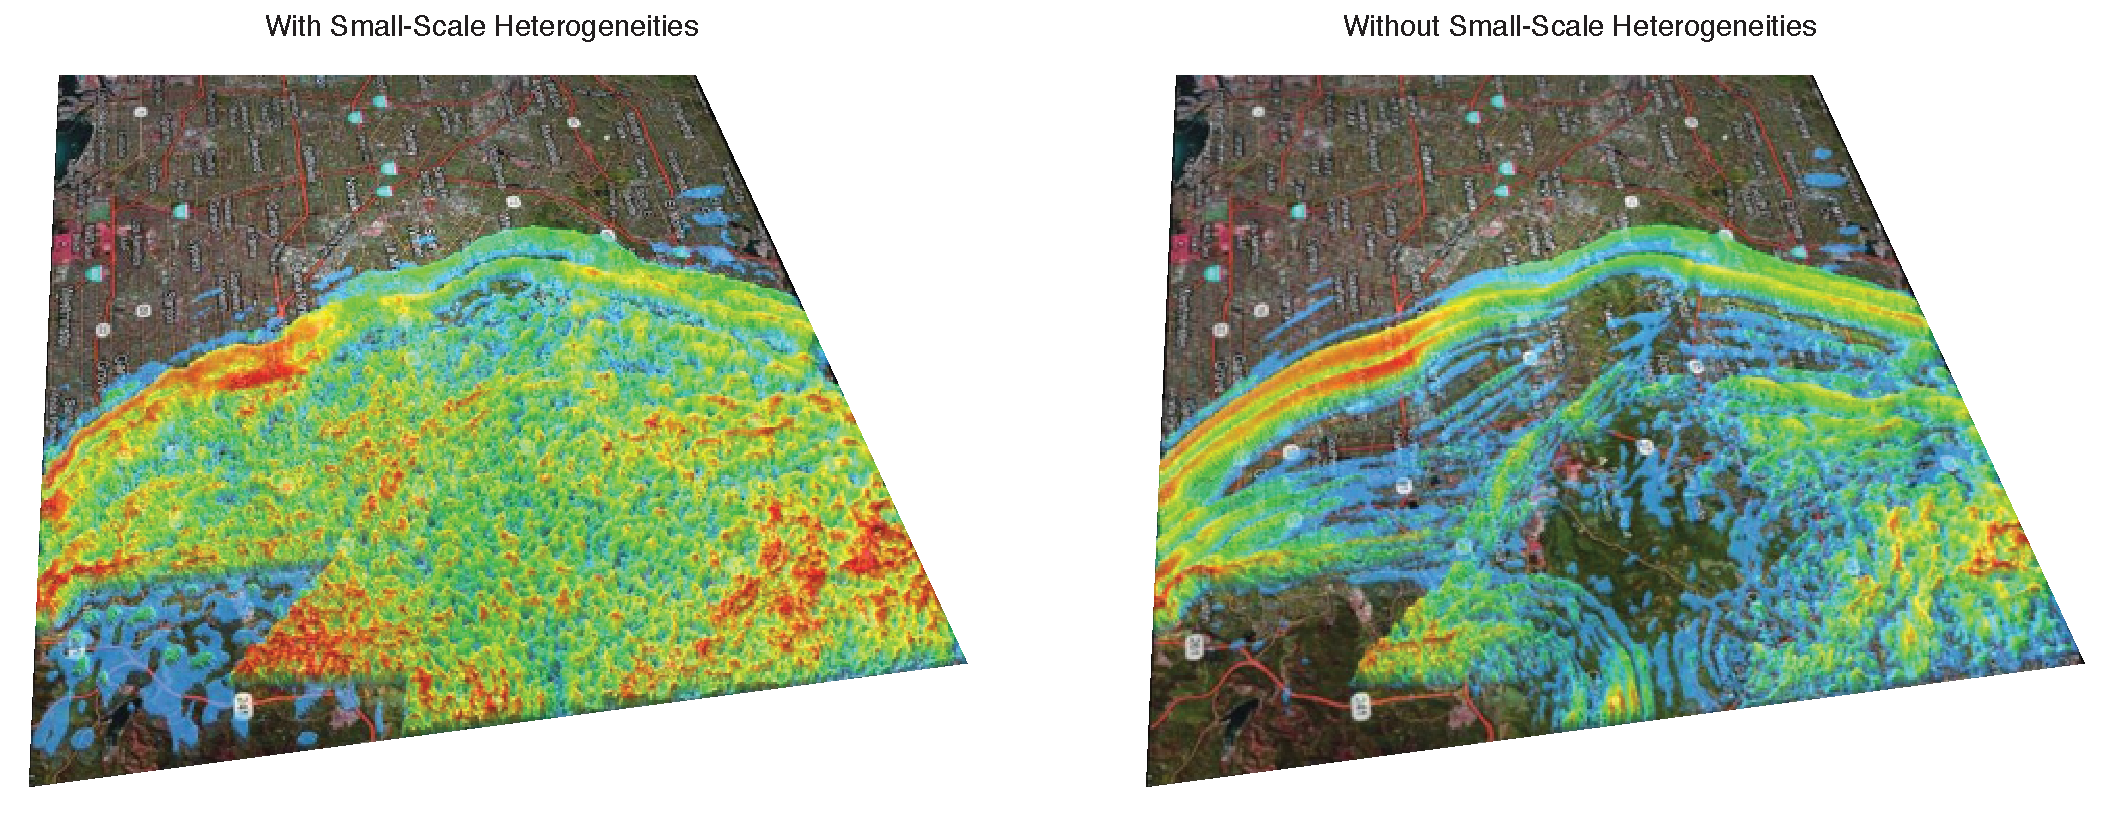
\includegraphics
        [width=0.80\textwidth]
        {figures/pdf/heterogeneities}
    \caption{Comparison of snapshots of velocity magnitude for simulations of the 2008 \eqmag{w} 5.4 Chino Hills, CA, earthquake, in subsets of the CVM-S V4 (left) with and (right) without a Von Karman distribution of small-scale heterogeneities.}
    \label{fig:heterogeneities}
\end{figure*}
